\subsection{Grayscale to RGB}
For our project we were provided with three SEVIRI visible channels: VIS 0.6, VIS 0.8, IR 1.6 %(reference p7 in summary of kit doc sent by Frazer) 
from METSAT 9. Channel wavelengths were centred on 0.635 $\mu$m [0.56-0.71 $\mu$m], 0.81 $\mu$m [0.74-0.88 $\mu$m] and 1.64 $\mu$m [1.50-1.78 $\mu$m] respectively, (p9) where the bracketed ranges show the spectral bandwidths of each channel. 
\par The first step required for analysis of this data was the visualisation of the channels provided, both individually and as an RGB image. The construction of an RGB image requires three channels, one representing the red spectra, one for the green and the final one for the blue. The channels given were not provided in this format and we therefore had to select how to stack our three channels in place of the red, green and blue channels in a traditional image. Approximate wavelength ranges for the visible spectrum are given in nanometres by Red: 780 - 622, Orange: 622 - 597, Yellow: 597 - 577, Green: 577 - 492, Blue: 492 - 455 and Violet: 455 - 390 %(reference website url https://www.livephysics.com/physical-constants/optics-pc/wavelength-colors/, can use better reference than if found I just picked one that seemed reliable?). 
From these values we determined that the nearest approximation of these channels with the 3 channels we have access to is Red: IR 1.6, Green: VIS 0.8, and Blue: VIS 0.6. 
\par For a desired datetime the images were searched for the corresponding channel files, which were subsequently selected and read into numpy arrays. These three arrays were then stacked in the order defined above, before being displayed as an RGB image as shown in Fig.~\ref{}. To obtain a more accurate RGB image, a weighting can be added to each channels values to adjust for the difference in channel wavelength values. 
\subsection{Cloud Removal}
 Before analysis can be done on satellite data to track changes in vegetation, crop growth, deforestation and sea temperature etc, the cloud cover obscuring the surface must first be taken into account and removed. There are a number of ways of doing this, a couple of which we explored and compared in our project. 
\subsubsection{Averaging Pixel Values}
 One of the simplest but most ineffectual ways of obtaining a cloud free image is to calculate an average image using multiple images centred over the same area on the Earth's surface. This works by assuming that there are a greater number of images with cloud free areas and that these cloud free pixels will reduce the influence of the cloudy pixels in the final image. The effectiveness of this technique very much depends on the ratio of cloud free days to covered ones and may also introduce cloudy pixels to areas that were previously cloud free. To illustrate this we plotted an averaged image by stacking multiple images together in four dimensions and averaging over the pixel values for each RGB channel as shown in Fig.~\ref{}. This image demonstrates why it is preferable to use other methods of cloud cover removal before further analysis of the image, as the image obtained still contains areas of cloud cover that prevent easy analysis of the terrain.
% Did we just straight up average over the images ? I can do if we haven't and we want it in the report to demonstrate why thresholding and masking is necessary and why we can't just average pixels over multiple days. 
\subsubsection{Thresholding Via Inspection}
 A common method of cloud cover removal makes use of thresholding to determine the cloudy and non-cloudy pixels. Thresholding allows an image to be split into two or more regions based on given threshold values. It works by setting all values above the chosen threshold to one value and all values below the threshold value to another, either 1 or 0 depending on which section of the image is desired as shown in Eq.~\ref{eq:thresh}.
 \begin{equation}\label{eq:thresh}
     g(x,y)=\Big\{\begin{matrix}
1 & if~f(x,y)~>~ T\\
0 & otherwise
\end{matrix}
 \end{equation}
 In the case of multiple threshold values it is the ranges between these values that have the same value assigned to them. Thresholding an image results in a binary image that can then be used as a mask to select the desired parts of an image and hide other areas. The differing cloud and surface level pixel values in the VIS 0.6 and VIS 0.8 channels meant that we were able to set threshold values to create masks to cover (and therefore remove) the cloud cover from our images. Due to the variation in the pixel values across the Earth's surface depending on latitude and longitude, a smaller area of 200x200 pixels was selected upon which to apply this cloud removal method. The threshold values were initially chosen via inspection of the RGB pixel values of the cloudy pixels in the plotted RGB image and were further adjusted once the masks were applied. This was done by setting threshold ranges for each RGB channel and creating a two dimensional mask array of ones,  in which the pixel's were set to 0 if the corresponding pixels fell within the threshold ranges in all three channels. A three dimensional mask was then created by stacking three copies of the two dimensional mask, which was then multiplied element wise with the RGB image channels to produce a cloud free image as shown in Fig.~\ref{}. 
 
\subsubsection{Otsu's Method for Thresholding}
\begin{figure}
\centering
    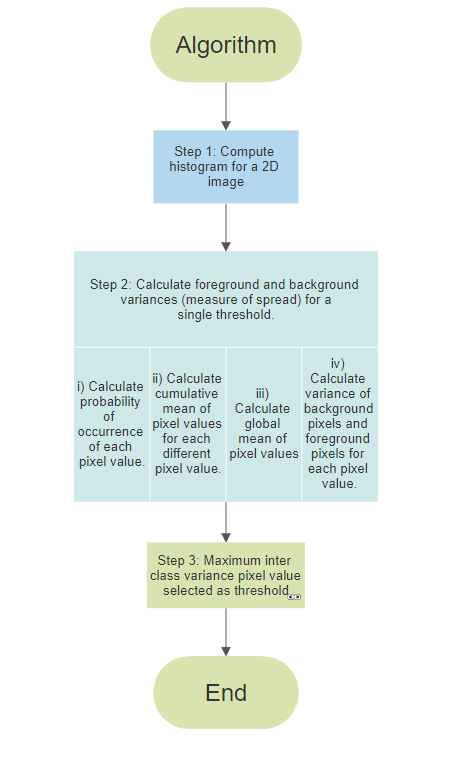
\includegraphics[width=0.6\textwidth]{flowchart_otsu.png}
    \caption{\label{diagram}}
\end{figure}

As can be seen in Fig.~\ref{} although the threshold values chosen were successful at removing most of the cloud cover there are still areas where cloudy pixels are present and better threshold values are required to remove these. There are multiple methods that analytically determine "optimum" threshold values for image segmentation based off of different definitions of goodness. One such method is Otsu's method. This is an automatic global thresholding technique that calculates the optimum threshold values for each image so that the measure of separability is maximised and the spread of pixel levels is minimised for the foreground (cloudy) and background (cloud free) pixels.



\begin{equation}
p_{i}=\frac{n_{i}}{M N}
\end{equation}


\begin{equation}
P_{1}(k)=\sum_{i=0}^{k} p_{i}
\end{equation}

\begin{equation}
m(k)=\sum_{i=0}^{k} i p_{i}
\end{equation}


\begin{equation}
\sigma_{B}^{2}(k)=\frac{\left(m_{G} P_{1}(k)-m(k)\right)^{2}}{P_{1}(k)\left(1-P_{1}(k)\right)}
\end{equation}

\subsubsection{Neural Networks and Deep Learning}

\subsection{Cloud Detection}
\subsubsection{Image Segmentation}

\subsection{Terrain Identification}
% A measure of
\subsection{River Identification}



